\chapter{\Des}
\inline{sammenligning af simulation vs. modellering.\\
  simulering er en implementation af modellen.\\
  styrke er samspillet mellem flere elementer/modeller.\\
  simulering - dynamisk - tid (time/space).} 

Simuleringer har længe været et værdifuldt værktøj til at klarlægge hvordan et 
system fungerer og er specielt brugbart til at repræsentere systemer hvis 
tilstand ændres over tid, eller såfremt der er interaktion mellem flere systemer. En 
matematisk model af disse systemer vil ofte være væsentligt mere kompleks og 
kan være svær at overskue lige så let som en simulering af samme system. 

Simuleringer foretages ofte af andre videnskabsfolk end dataloger, og det er 
derfor vigtigt at de kan repræsenteres i et sprog som er let tilgængeligt og 
minimerer sandsynligheden for at begå fejl i konstruktionen af simulationen.  
Til dette formål er programmeringssproget Python oplagt da det netop fokuserer 
på let tilgængelighed og høj produktivitet for udvikleren. 

Det er oplagt at benytte CSP\cite{hoare-csp} til at repræsentere en simulering.  
I CSP er interaktionen mellem forskellige processer/systemer eksplicit, og på 
grund af modulariteten er det nemt at konstruere komplekse systemer ud fra 
mindre, enkle systemer. 

%\section{Beskrivelse/teori} \label{sec:des-teori}\fxnote{Dårlig overskrift?}
%\inline{Beskrivelse af tidsmodellen, teorien omkring den og hvor/hvad den 
%    benyttes til. Teori: henvisning til litteratur, bl.a.  matematik/beviser 
%    for modellen}
%\inline{Skal vi skrive noget om at introduktionen af tid er det samme som at introducere prioritet}

%\pdfcomment{Jeg synes der mangler en tydelig defintion af sikret tid}
%\inline{Gennemlæses og højst sandsynligvis omskrives med henblik på sammenhæng og mangler.}
%Inden for simulering er \des en meget brugt metode til at modellere systemer. I 
%\des anskues tid som \kv{diskrete tidsskridt}, som er uden kobling til realtid. I disse tidsskridt udføres en eller flere begivenheder, som hver især ændrer på systemets tilstand. Når alle begivenheder for et tidsskridt er udført, kan tiden tælles op, og begivenheder for det nye tidsskridt kan udføres. Der kan være fastlagt et vilkårligt antal begivenheder til et tidsskridt, og hver begivenhed kan variere vilkårligt, ifht., hvor langt tid den tager at udføre i realtid. Dermed er der ikke nogen kobling mellem den diskrete tid og realtid, og et diskret tidsskridt kan variere vilkårligt i realtid. Begivenhederne, der skal udføres af systemet, kan enten være givet på forhånd eller blive skemaplanlagt dynamisk under afviklingen af andre begivenheder. 
%Afhængig af hvad der simuleres, kan man udtrække relevant information om systemet f.eks. gennemsnitlig behandlingstid for elementer, længden af køer i systemet og den samlede aktivitetstid for hvert delelement i systemet.

%For at kunne konstruere en \des skal vi have følgende til rådighed: \pdfcomment{Hvorfor er dette ikke først i afsnit 2.1}
%\begin{enumerate}
%\tightlist 
%\item En repræsentation af tid til at styre, hvornår vi skifter tidsskridt.
%\item En liste over begivenheder, der skal udføres i hvert tidsskridt.
%\item Mulighed for at opsamle statistisk data fra simulationen. 
%\end{enumerate}
%En repræsentation af diskret tid skal kunne udtrykke den aktuelle tid, \ikkef{endelig fremtidig tid} og gerne kunne foretage en variabel fremskrivning af tiden. Eksempelvis kan man forestille sig, at der \ikkef{i tiden $t_{0}$ planlægges en begivenhed til tiden $t_{3}$}. Såfremt der ikke er planlagt andre begivenheder, er det her en fordel at kunne springe over $t_{1}$ og $t_{2}$ og fremskrive tiden direkte til $t_{3}$. \pdfcomment{Dette er om 1, men der står intet skrevet om 2 og 3}



%I \csp har vi garanti for at de eneste afhængigheder mellem processer vil være kommunikation. I \des har vi ud over kommunikation også en afhængighed af at synkronisere tiden mellem processerne. 

%En simulering løber begivenhederne kronologisk igennem til der enten ikke er flere begivenheder eller som det oftere er tilfældet til simuleringen når et forud defineret tidspunkt.
\subsubsection{PDES}
\fxnote{skriv lidt mere om hvad pdes er}
Et alternativ til \des  er parallel discrete event simulation(\pdes) hvor tiden i processerne kan løbe uafhængigt af hinanden. Dette introducerer muligheden for større parallellitet, men samtidigt risikerer processerne ved kommunikation at modtage beskeder fra fortiden, som der skal tages hånd om, f.eks. ved at rulle tiden tilbage. \pdes har ikke vundet stort indpas i den videnskabelig verden, som man kan se af \cref{tab:des}. En grund til dette er, at når tiden kan køre parallelt, øges omkostningerne for at kunne rulle tiden tilbage, hvilket resulterer i lavere hastighed, end når tiden holdessynkront på tværs af processerne.

\begin{table}[ht]
	\centering
	\begin{tabular}{lrr}
	\toprule
	\mc{Periode} & \mc{DES} & \mc{PDES}\\
	\midrule
1970 til 1980 &   296 &2\\
1980 til 1990 & 1.460 &95\\
1990 til 2000 & 6.190 &1.260\\
2000 til 2010 &13.100 &1.210\\
\bottomrule
	\end{tabular}
	\caption{Publisering af artikler if. google scholar ved søgning på hhv. ``discrete event simulation'' og ``parallel discrete event simulation''}
	\label{tab:des}
\end{table}
%\subsection*{Noter til afsnittet}
%\begin{itemize}
%\tightlist
%	\item stokastisk varians i relation til M/M/1
%	\item Hvad bruges DES til? styrker/svagheder?
%	\item Henvis til DE-simulation.ps
%  \item Eksempel på problemer som løses med des
%  \item model vs. simulering
%\end{itemize}


\subsubsection{Barrierer} \label{sec:barrierer}
%\inline{Hele afsnittet skal skrives om for at få det generelle samlet i starten, og vores specifikke efterfølgende. Evt. have mindre om vores implementation}

I \des findes en \fxnote*{skal defineres?}{global tid}, og alle processerne skal derfor have en fælles tid, der tæller op 
samtidigt.  En global viden som tid kræver synkronisering af alle 
processerne, og til denne koordinering og synkronisering af flere 
processer er  den mest brugte metode at introducere en barriere. Barrierer blev først introduceret i MPI \cite{mpi-barrier}, hvor den bruges til at 
sikre, at alle tråde venter i barrieren før de  fortsætter. 

I \csp kan man lave sin egen barriere ved at udnytte, at begge 
kanalender skal være klar, før der kan kommunikeres, og at en proces, der 
indgår i en kommunikation, derfor vil vente indtil den anden ende er klar. Ved hjælp af kanaler kan man derfor lave en simpel barriere 
 ved brug af kommunikation over kanaler.  En implementering af den simple 
barriere som en selvstændig proces kan ses i \cref{barrier-imp}.

\begin{lstlisting}[float, label=barrier-imp,caption=En barriere i \pycsp]
@proces
def Barrier(nprocesses, signalIN, signalOUT):
	while True:
		for i in range (nprocesses):
			signalIN()
		for i in range (nprocesses):
			signalOUT(0)
\end{lstlisting}
%
%Denne implementering af en barriere kræver, i modsætning til de fleste andre 
%implementeringer af barrierer\cites{mpi-barrier, crew}, to kald. Det første 
%sender en variabel til barriereprocessen, mens,
%det andet kald modtager en dummyværdi fra barriereprocessen. Det kræver derved 
%to kanaler at implementere barrieren. På den ene kanal er barrieren den eneste 
%der læser værdierne; en besked sendt på denne kanal vil derfor altid modtages 
%af barrieren. På den anden kanal er barrieren den eneste der skriver, og en 
%modtaget besked må derfor komme fra barrieren.
%
%Vi kan overbevise os om korrektheden af barrieren, da alle processerne først 
%går ind i barrieren ved at sende en værdi til barrieren. Hvis barrieren ikke er 
%klar, sikrer \csp at processerne venter indtil barrieren er klar til at modtage 
%værdierne. Først når barrieren har modtaget en værdi fra alle processerne, 
%begynder barrieren at sende sin værdi, og det er først når en proces modtager 
%denne værdi fra barrieren at den må fortsætte. Når en proces modtager værdien 
%fra barrieren fortsætter den og man kan risikere at den ønsker at gå ind i 
%barrieren inden denne har sendt sin værdi til alle processer for at frigive dem.
%Processer der ønsker adgang til barrieren vil da gå i stå, idet de prøver at 
%sende til barrieren før den er klar til at modtage. Først 
%når barrieren har signaleret til alle processer at de må fortsætte, læser den 
%på kanalen for at accepterer processer der ønsker at tilgå barrieren. Det er 
%denne egenskab fra \csp der giver os garanti for at en proces der netop er 
%frigivet fra barrieren ikke går ind i den igen og derved risikerer at komme 
%foran. 
%
%En ulempe ved denne simple barriere er at antallet af processer skal være 
%konstant gennem hele kørslen.
%Vi vil senere se på et bankeksempel hvor dette problem opstår (\cref{bank-eksempel}). Her ville nogle af 
%processerne kunne slutte tidligt, men må fortsætte med  at kalde barrieren, indtil alle processerne er klar til at slutte.
%Man kunne ændrer barriereprocessen, så man dynamisk kan ændre på antallet af processer der 
%skal synkroniseres. I de fleste implementationer af barrier er dette en mulighed, men til vores simple illustration, har vi valgt ikke at implementere det.

Barrierer er en meget effektiv metode til at synkronisere processer, der kører 
parallelt, og er brugt flittigt i MPI. I \csp findes der dog en konflikt i brugen 
af barrierer, selvom det er nemt at implementere. Problemet er at hver proces bør fungere i isolation, og den eneste interaktion mellem processerne er via kanalerne. Derfor virker introduktionen af barrierer og kald til disse kunstig i \csp. 

\citeauthor{crew} beskriver brugen af barrierer som:
\begin{otherlanguage}{english}
\mycite[1]{crew}{[\ldots] where the barriers may be used to maintain global and/or localised models of time and to synchronise safe access to shared data[\ldots]}
\end{otherlanguage}
Barrierens berettigelse i CSP er derfor at  introducere tid og at kunne bruge delt data. I \csp bør der ikke være delt data mellem processerne, men derimod kun lokalt data. Hvis data er delt pga. den arkitektur \csp er implementeret på, bør dette abstraheres væk og udnyttes internt i kanalerne. At introducere hjælpemidler for at styre delt data, er derfor at tilskynde til en forkert brug af \csp. Tiden er den anden begrundelse for at benytte barrierer.
Men barrierer giver kun en  primitiv model for tid, og vi vil vise, at med brugen af \des får man et stærkere værktøj, der blandt meget andet også kan erstatte brugen af barrierer.

\subsubsection{Timeout} 
I den eksisterende \pycsp findes der som nævnt i \autoref{sec:csp} en \code{alternation}, hvor brugeren har mulighed for at tilknytte to specielle guards. Den ene er en SKIP-guard, der giver mulighed for at kommunikere, hvis kanalen er klar og ellers fortsætte uden at kommunikere. Den anden er timeout-guarden, der udvider SKIP-guarden så man venter på kommunikation i en given periode hvorefter man tager SKIP-guarden. 
Når \des indføres, ændres tiden, så timeout-guarden opererer på tidsskridt fremfor en tidsperiode. Vi går derved fra en situation hvor en timeout-guard f.eks. er villig til at vente i fem sekunder, til at den nu er villig til at vente i 5 tidsskridt. Denne ændring virker umiddelbart simpel, men introducerer et problem i forhold til hvornår timeout-guarden vælges. En proces kan nu ønske at kommunikere i indeværende tidsskridt men ikke i det efterfølgende. Vi kan dog ikke i tidsskridtet evaluere om kommunikation er muligt. Dette skyldes, at tiden står stille mens processerne er aktive, så selvom kommunikation ikke er muligt på ét tidspunkt i tidsskridtet, så kan en efterfølgende begivenhed i samme tidsskridt muliggøre kommunikation.

En løsningsmodel på denne problemstilling kunne være at lade processer i timeout-guards vente helt frem til næste tidsskridt, og her lade dem vælge SKIP-guarden. Dette efterfølgende tidsskridt kan enten være et ekstra skridt, vi introducerer specifikt for at håndtere disse timeout-guards, eller det kan være det næste tidsskridt, hvortil der er planlagt en begivenhed. 
Såfremt vi introducerer et kunstigt tidsskridt skal dette specificeres i definitionen af timeout-guarden. Uanset hvor lille et tidsskridt vi specificerer, kan vi ikke garantere, at der ikke efterfølgende, i samme tidsskridt, vil blive planlagt en begivenhed til at indtræffe mellem indeværende tidsskridt og det kunstige tidsskridt, vi specificerede i timeout-guarden. Herved er der risiko for, at rækkefølgen af begivenheder, der skal udføres bliver ændret, hvilket er uacceptabelt. 
Alternativt kan man vælge at lade tiden springe til den næste begivenhed, der er planlagt, og der som det første vælge SKIP-guarden. Her vil man ikke risikere at ændre på rækkefølgen, men derimod at springe for langt frem i tiden. Dette kan være et problem, hvis en proces, der tager en SKIP-guard, efterfølgende planlægger en begivenhed.
Begge muligheder har grundlæggende den svaghed, at oprindeligt ønskede man kun at kommunikere i det indeværende tidsskridt og ikke i hverken et vilkårligt lille tidsrum eller i et tilfældigt tidsrum frem til en efterfølgende begivnhed.

En sidste løsningsmodel er at vente til lige før, tiden tælles op, og der kalde de ventende processers SKIP-guards. 
For at kunne adskille hvilke processer, der har en begivenhed til et tidsskridt, og hvilke, der venter på kommunikation, kan vi \fxnote*{illustration}{benytte os af edge-triggering} til at dele hvert tidsskridt op i to grupper, henholdsvis wake-first og wake-last.
I wake-first-gruppen udføres de processer, der har tilknyttet en begivenhed til det givne tidsskridt, mens man i  wake-last-gruppen aktiverer SKIP-guarden for de processerne der venter på en timeout.

Edge-triggering er den bedste løsningsmodel af de beskrevne, da man her har mulighed for at udføre alle begivenheder, som måske resulterer i kommunikation, og først derefter aktivere SKIP-guards, for de processer der har en timeout til samme tidsskridt. Ulempen ved denne metode er at det krævere en mere kompleks implementering, da der nu findes to seperate måde at vente for hhv. begivenheder og timeouts.


\chapter{Eksempler}

\section{Hajer og fisk på Wator} Som eksempel på en DES simulation
har vi valgt at tage udgangspunkt i det scenarie som A. K. Dewdney
beskrev i artiklen \fixme[inline]{reference}. Artiklen beskriver den
fiktive planet Wator, der har form som en torus og er fuldstændig
dækket af vand. Verdenen er inddelt i felter som beskrevet på side
20 i \fixme[inline]{ref}. Disse felter kan være tomme, indeholde en
fisk eller en haj. Følgende karakteristika beskriver fisk og hajers
opførsel.


Fisk - bevæger sig og forplanter sig Lever af plankton, en ressource
som er uendelig. Hvis der er et ledigt tilstødende felt bevæger en
fisk sig til dette felt. Hvis der er flere ledige felter vælges et
tilfældigt. Hvis en fisk overlever 3 livscykler forplanter den sig.


Hajer - jager og forplanter sig Såfremt der er fisk i et eller flere
tilstødende felter flytter hajen sig herhen og spiser fisken. Hvis der
er flere tilstødende felter med fisk vælges et tilfældigt. Er der
ikke nogen fisk i nærheden bevæger en haj sig på samme måde som en
fisk. Hvis en haj ikke spiser i mere end 3 livscykler dør den. Hvis en
haj overlever 10 livscykler forplanter den sig.

For hvert tidsskridt vil alle fisk og hajer udføre en handling ud fra
ovenstående opførsel.

Til at initiere systemet skal der defineres en størrelse af verdenen,
samt hvor mange fisk og hajer der er til stede fra start. Disse fisk og
hajer placeres tilfældigt i verdenen.

Såfremt de initielle parametre understøtter en bæredygtig bestand
forventer vi at se bestanden af henholdsvis fisk og hajer oscillere
afhængigt af hinanden.

\section{Kunder i en bank} Et klassisk eksempel inden for \des


\section{Design og implementering}
%\inline{Beskrivelse af design med udgangspunkt i eksemplet}
For at designe en implementering af simulering i diskret tid i \pycsp, skal vi foretage en række ændringer i forhold til den nuværende implementering. Specifikt skal vi ændre på planlægningen og eksekveringen af processer, hvortil vi har brug for at kunne repræsentere en diskret tidsmodel. Vi vil i dette afsnit gennemgå de relevante problemstillinger og løsningsmodeller samt give et overblik over, hvordan vi har valgt at implementere ændringerne rent praktisk i koden. 


\subsection{Kodestruktur}  
Efter i kapitel \ref{chap:csp} at have valgt at udvide \emph{greenlets}"-versionen, skal vi vælge hvordan vi ønsker at videreudvikle koden. Vi forventer at genbruge store dele af koden fra \emph{greenlets}"-versionen, og kun foretage udvidelser på enkelte afgrænsede områder. Desuden ønsker vi at isolere vores ændringer fra den originale \emph{greenlets}"-versionen. Med denne isolation forventer vi, at hvis/når der sker tilrettelser af \emph{greenlets}"-versionen af \pycsp, vil man ikke skulle foretage de samme tilrettelser i vores version. 
Isolationen mellem de to versioner skal opnås via nedarvning, således at det fra en brugers synsvinkel ser ud til, at vores version er fuldstændigt sepereret fra \emph{greenlets}"-versionen.

Hver af de tre versioner har sin egen mappe i \pycsp og i hver af disse findes en tilhørende \code{\_\_init\_\_.py} fil, der fungerer som et manifest for den givne version. Vi opretter vores egen version kaldet \emph{simulation} og opretter også en tilhørende mappe på samme niveau som de andre versioner og med sin egen manifestfil. Manifestfilen kan nu bruges til at udvælge de funktioner, der skal tages direkte fra \emph{greenlets}-versionen, og hvilke funktioner, der skal udvides og som derfor vil ligge i den nye mappe.

\begin{lstlisting}[float=hbtp,label=fig:init,caption=Uddrag af \code{\_\_init\_\_.py} for simulationsversionen.]
from guard import Timeout, Skip
from pycsp.greenlets.alternation import choice
from alternation import Alternation
from pycsp.greenlets.channel import ChannelPoisonException, ChannelRetireException
\end{lstlisting}

I \cref{fig:init} kan man se, at funktionerne \code{choice}, \code{ChannelPoisonException} og \code{ChannelRetireException} alle bliver hentet fra \emph{greenlets}"-versionen, mens funktionerne \code{Timeout, Skip} og \code{Alternation} bliver importeret fra samme mappe og derfor er modificerede versioner. For slutbrugeren  vil dette dog ikke være synligt, og han vil blot se \emph{simulation}"-versionen som en selvstændig version på lige fod med de andre tre versioner.

\subsection{Scheduler-klassen}
\label{sec:scheduler}
Med valget af \emph{greenlets}"-versionen som grundversion, og med henblik på at hovedparten af vores ændringer vil være i \sched en, vil vi kort gennemgå dele af klassen \code{Scheduler}.

\begin{lstlisting}[firstnumber=132,stepnumber=5,numbers=left, float, label=fig:scheduling, caption=Uddrag af Scheduler.py i \emph{greenlets}versionen.]
    def getInstance(cls, *args, **kargs):
        '''Static method to have a reference to **THE UNIQUE** instance'''
        if cls.__instance is None:
            # (Some exception may be thrown...)
            # Initialize **the unique** instance
            cls.__instance = object.__new__(cls)

            # Initialize members for scheduler
            cls.__instance.new = []
            cls.__instance.next = []
            cls.__instance.current = None
            cls.__instance.greenlet = greenlet.getcurrent()

            # Timer specific  value = (activation time, process)
            # On update we do a sort based on the activation time
            cls.__instance.timers = []

            # Io specific
            cls.__instance.cond = threading.Condition()
            cls.__instance.blocking = 0
\end{lstlisting}

 I \cref{fig:scheduling} ses et uddrag af initialiseringskoden, der er interessant, fordi det er her alle de interne datastrukturer oprettes. Man kan her se de tre lister af processer, som \sched en har til rådighed til at varetage processkifte. 
 \begin{list}
 \tightlist 
 \item \code{new}: Initieres på linje 140 og består af processer, som lige er blevet planlagt for første gang. Nye processer kan ankomme til listen \code{new} via funktionerne \code{Parallel, Sequence} og \code{Spawn}.
 \item \code{next}: Initieres på linje 141 og indeholder de processer, der er klar til at blive kørt, og som har været kørt på et tidligere tidspunkt. Et eksempel kunne være en proces, der har stoppet sin kørsel for at vente på kommunikation. Processen vil blive placeret i denne liste, når kommunikationen er overstået. 
 \item \code{timers}: Initieres på linje 147 og indeholder de processer, der har tilknyttet en timeout. De skal først planlægges på et senere tidspunkt og venter dermed blot. Hvert element i listen består både af processen samt et tidsstempel for hvornår processen skal genaktiveres. 
 \item \code{blocking}: Initieres på linje 151 og er en variabel. Processer, der venter på IO-operationer, er ikke klar til at blive planlagt, men heller ikke afsluttet. \Sched en kan derfor ikke planlægge dem, men holder styr på antallet af ventende processer vha. denne variabel. Dette bruges bla. for at kunne afgøre om \sched en har planlagt alle processer.
\end{list}

Når \sched en er startet, gennemløber den alle tre lister gentagne gange, indtil de alle er tomme, og der ikke er nogle processer, der er blokeret. Dette betyder at der ikke længere kan komme nye processer til der ønsker at blive lagt på \sched en, og dermed kan den afslutte.

For at markere at vi ikke kun skal  planlægge rækkefølgen
af processerne, men også styre tiden, har vi lavet en
\code{Simulation}"-klasse, der arver fra \code{Scheduler}"-klassen. Alle ændringer
vi skal foretage for at kunne planlægge processer under hensyntagen til tid, vil således være indkapslet i denne klasse. 
Dette har yderligere den fordel, at man tydeligt kan se at alle klasserne i \code{simulation}-versionen arver en \sched~ fra \code{Simulation} og
ikke en \sched \xspace fra \code{greenlets}-versionen.

\subsection{Tid} \label{sec:tid}
For at kunne planlægge begivenheder i \des kræves det at alle processer og \sched en har en global forståelse af tid.  Det er derfor en af hjørnestenene i implementeringen af \des, hvordan tid introduceres til \pycsp.  
Begrebet tid er ikke en del af \csp, men er alligevel blevet introduceret i \pycsp, for  at  kunne tilknytte en timeout til en \code{alternation}. Vi ønsker
at videreudvikle denne struktur til at håndtere tid generelt for alle
processer, og til at fungere med vores tidsmodel, modsat den eksisterende
løsning, hvor \code{time}-modulet benyttes.
 
\CRef{Timeout} viser et eksempel på brugen af tid i det eksisterende \pycsp, hvor en \code{alternation} er villig
til at læse fra kanalenden \code{Cin} i 0,5 sekunder. Hvis ikke der
er modtaget en besked indenfor 0,5 sekunder, accepteres dens \code{timeout-guard},
og processen fortsætter sin kørsel uden at have læst fra kanalen.

\begin{lstlisting}[float=hbtp, 
label=Timeout,caption=Timeout i Alternation (fra dokumentationen til PyCSP)]
Alternation([{Timeout(seconds=0.5):None}, 
             {Cin:None}]).select()
\end{lstlisting}

\inline{Dette skal gennemlæses når deadline/interactive  er skrevet for at se om time modulet skal hives op på et højere niveau}

Fra en brugers synsvinkel repræsenteres tiden internt i \pycsp som realtid, men dette er ikke korrekt. Helt generelt kan computere ikke håndtere kontinuerlige begreber, som realtid er, og \code{time}-modulet, der står for håndtering af tid i Python og dermed \pycsp, kan derfor ikke give brugeren mulighed for at benytte realtid. 

 I stedet tilbyder \code{time}-modulet det, vi vil kalde ``pseudo realtid'', der minder om realtid, men på en række områder afviger fra denne. Den største forskel mellem realtid og pseudo realtid er, at i computere kan tiden ikke være kontinuerlig, men må nødvendigvis være diskritiseret, og som oftest i et fast lille tidsskridt. Vi skal med vores diskrete tidsmodel derfor ikke foretage en konvertering fra kontinuerlig til diskret tid, men i stedet skal foretage en konvertering fra en diskret tidsmodel. hvor tiden stiger med et fast tidsskridt, til en diskret tidsmodel, hvor tiden stiger med variable tidsskridt. Vi skal desuden ændre fremskrivningen af tiden så den  drives af begivenheder og ikke af et eksternt modul i pseudo realtid. \fxnote{Kan vi ryste noget ud med hvorfor det er godt vi ikke skal gå fra kontinuerlig til diskret tid?}
 
 
\subsubsection{Sammenhæng mellem tidsintervaller i realtid og diskret tid}
Da man i \code{time}-modulet har et fast tidsskridt, og
realtiden også er inddelt i faste størrelser
som eks. sekunder, kan man med \code{time}-modulet måle tidsintervaller, der
korresponderer med realtiden. I \des findes der ikke en
sammenhæng til  realtiden, da tiden blot er et tal, der starter som 0, og stiger
i arbitrære tidskridt. Når tiden i \des på denne måde er afkoblet
en relation til realtid, giver det ikke mening at have elementer i simuleringen, der er afhængige af realtid. 
I \pycsp kan man planlægge en timeout til at ske om f.eks. 5 sekunder. I \des findes sekunder som
begreb ikke, men man  angiver i stedet, at når tiden er talt op med 5 tidsskridt, skal
begivenheden ske. Der findes dog ikke en total afkobling mellem tiden i \des og realtiden, for givet et konkret problem, der skal modelleres i \des, vil der altid være en sammenhæng mellem tiderne. Men da denne sammenhæng ikke er fast, skal den defineres eksplicit af brugeren, som f.eks at 5 sekunder i problemet defineres som en stigning i tiden med f.eks 5, 0,5 eller 0,05 i simuleringsmodellen.

Når tiden i \des er uafhængig af realtiden, er der ingen grund til at bruge en kompleks model af tiden, og vi har derfor valgt at repræsentere tiden som et positivt tal, der findes internt i \sched en. Dermed findes der kun en version af tiden, da  \sched en er en singelton. For processer, der ønsker at kende tiden, har vi
introduceret funktionen \code{Now}, der returnerer tiden fra \sched en, når funktionen kaldes. En fordel ved brugen af funktionen \code{Now} som en wrapperfunktion til at bede om tiden i forhold til den eksisterende kode, der direkte kalder \code{time}-modulet, er, at vi frigøres fra en konkret implementering af tid. For fremtiden er det kun funktionen \code{Now}, der skal omskrives, for at hele systemet bruger en anden implementering tid.

I den eksisterende kode har det ikke været tiltænkt, at man ønskede at udskifte implementeringen af tiden, vi skal derfor ændre de steder, hvor \code{time}"-modulet er refereret. Heldigvis bruges \code{time}-modulet kun ved udvælgelse af processer fra \code{timers}-listen (\cref{fig:green:timer}). 
\begin{figure}[hbtp]
\begin{minipage}[c]{\linewidth}
\begin{lstlisting}[firstnumber=204, label=fig:green:timer, caption=Udvælgelse af proces fra listen timers (fra scheduling.py)]
if self.timers and self.timers[0][0] < time.time():
  _,self.current = self.timers.pop(0)
  self.current.greenlet.switch()
\end{lstlisting}
\end{minipage}
\begin{minipage}[c]{\linewidth}
\begin{lstlisting}[firstnumber=124, label=fig:sim:timer, caption=Udvælgelse af proces fra listen timers (fra simulation.py)]
if self.timers and self.timers[0][0] <= Now():
  assert self.timers[0][0] == Now()
  _,self.current = heapq.heappop(self.timers)
  self.current.greenlet.switch()
\end{lstlisting}
\end{minipage}
\end{figure}
Her sammenlignes på linje 204 den første tidsværdi i \code{timers} med det nuværende tidspunkt givet af \code{time}-modulet.
Hvis det nuværende tidspunkt er større end værdien i \code{timers}, udvælges denne proces til at køre næste gang og fjernes fra listen.
For at planlægge begivenheder præcist, skal processerne kunne eksekveres på et specifikt tidspunkt. Dermed har  \sched en i \code{simulations}-versionen behov for at kunne  styre aktiveringen af processerne på et finere niveau end, hvad der er muligt med \code{greenlets}"-versionen.  
I \code{simulation}"-versionen har vi fuld kontrol over tiden, da  den står stille, mens processerne eksekveres, hvorfor dette ikke er et problem.
Vi  tilføjer den begrænsning, at tiden skal være præcist det, der er angivet i \code{timers}, før processen skal aktiveres, og ikke kun større, som angivet i \code{greenlets}-versionen. \CRef{fig:sim:timer} viser udvælgelsen af en proces fra \code{timers} i \code{simulerings}-versionen ved brug af \code{Now}-funktionen, hvor tidspunktet skal være præcist det som processen har angivet.

\subsubsection{Fremskrivning af tid}
I pseudo realtid drives tiden frem af et eksternt modul for at efterligne realtid, der kontinuerligt stiger. I pseudo realtid fremskrives tiden derfor uafhængigt af processernes tilstand og derfor vil et program der med korte mellemrum beder om tiden, få et stigende tidspunkt. I \des  skal tiden i modsætning til realtid stå stille, når processerne er aktive, og kun i forbindelse med en planlagt begivenhed skal tiden drives frem til tidspunktet for denne begivenhed.

\fxnote*{skriv tegning}{Vi kan demonstrere, hvordan den kontinuerlige tid har indflydelse på  \pycsp med et eksempel}. Proces 1 har startet en ny tråd via \code{io-decoratoren} og er derfor blokeret. Proces 2 står i en \code{alternation} med en \code{timeout-guard}. Uafhængigt af den tid, det tager proces 1 at komme ud fra sit blokerede kald, skal proces 2 vide hvornår dens timeout er indtrådt. Dette er implementeret i \code{greenlets}-versionen i \cref{fig:blocking_sleep} på linjerne 242 til 251. Her startes en separat tråd, der vil signalere til \sched en, når tiden for næste begivenhed i \code{timers} listen indtræffer. \Sched en kan nu nøjes med at vente på et signal, som vil komme fra enten en blokeret proces eller den nyoprettede tråd.

Når tiden i \des ikke er drevet af en eksternt modul, er nødvendigheden af en ekstra tråd til  håndtering af tid irrelevant. Først når alle begivenheder til et tidsskridt er eksekveret, skal tiden i \des tælles op. Dette betyder i vores konkrete eksempel, at  så længe proces 1 er blokeret, står tiden stille, og  \sched en venter på dem. Vi kan ikke tælle tiden op, blot fordi nogle processer er blokeret af \code{io-decoratoren}, ligesom vi ikke kan tælle tiden op, blot mens nogle processer eksekvere en anden tilfældig funktion.

Først når alle processer venter i enten \code{timers} listen eller på kommunikation, kan der ikke ske flere begivenheder og tiden sættes op. 
I dette tilfælde  kan \sched en finde tidspunktet for den begivenhed, der ligger tættest på det nuværende tidspunkt,  og springe frem til denne begivenhed. Dette er implementeret i \cref{fig:sim_sleep}.
\begin{figure}[hbtp]
\begin{minipage}[c]{\linewidth}
\begin{lstlisting}[firstnumber=239, label=fig:blocking_sleep, caption=Uddrag af \sched en i \code{Scheduler}]
self.cond.acquire()
if not (self.next or self.new):
    # Waiting on blocking processes or all processes have finished!
    if self.timers:
        # Set timer to lowest activation time
        seconds = self.timers[0][0] - time.time()
        if seconds > 0:
            t = threading.Timer(seconds, self.timer_notify)
            # We don't worry about cancelling, since it makes no 
            # difference if timer_notify is called one more time.
            t.start()
            # Now go to sleep
            self.cond.wait()
    elif self.blocking > 0:
        # Now go to sleep
        self.cond.wait()
    else:
        # Execution finished!
        self.cond.release()
        return
self.cond.release()
\end{lstlisting}
\end{minipage}
\begin{minipage}[c]{\linewidth}
\begin{lstlisting}[firstnumber=158, label=fig:sim_sleep, caption= Uddrag af \sched en i \code{Simulation}]
self.cond.acquire()
if not (self.next or self.new):
  # Waiting on blocking processes
  if self.blocking > 0:
    # Now go to sleep
    self.cond.wait()
  #If there exist only processes in timers we can increment
  elif  not (self.next or self.new or self.blocking): 
      if self.timers:
          # inc timer to lowest activation time
          self._t = self.timers[0][0]
      else:
          # Execution finished!
          self.cond.release()
          return
self.cond.release()  
\end{lstlisting}
\end{minipage}
\end{figure}


\subsection{Funktionen Wait}\label{sec:Wait}
Vi har valgt at anskue planlægningen af en begivenhed til et bestemt tidspunkt, sådan at den proces der skal udføre begivenheden venter indtil tiden for begivnheden er nået, og først her begynde udførslen. Dette vil i praksis være det samme som en planlægning til tidspunktet men det letter implementeringen da vi ikke behøver nogen viden om specifikke begivenheder i vores \sched. 

\begin{lstlisting}[firstnumber=11 , stepnumber=2, numbers=left,float=hbtp, label=fig:simpy:yield, caption= Et yield i \simpy (taget fra Bank05.py i eksemplet fra \simpy)] 
def visit(self,timeInBank): 
  print now(), self.name," Here I am" 
  yield hold,self,timeInBank print now()
  self.name," I must leave" 
\end{lstlisting}
I programmeringssproget \simpy benytter man også denne metode med at lade en proces vente. Dette gøres ved at
foretage kaldet \code{yield}, som sørger for, at processen ikke
fortsætter, før et defineret tidsrum er gået. \CRef{fig:simpy:yield} viser, at en kunde er ankommet til banken, hvorefter kunden printer tiden, foretager et \code{yield}, printer tiden igen og afslutter.  Når processen har kaldt \code{yield}, er tiden steget med værdien af \code{timeInBank}. Grunden til at \simpy kan bruge \code{yield}, der er indbygget i Python og at dette kald afgiver kontrol over processen i et tidsrum, knytter sig til deres implementering af \simpy, hvor de bruger \code{corutine} som underliggende teknologi. Som standard kan  \code{corutine} afgive kontrollen med en proces via \code{yield}, og \simpy behøver derfor kun at sikre, at tiden er talt tilstrækkeligt op, før de returnerer til processen.

 Vi ønsker i \pycsp at have en lignende mulighed for at lade en proces vente. Med \code{greenlet}-modulet af brugertråde kan vi ikke bruge \code{yield}, da denne er specifik for \code{co-rutines}, men funktionaliteten er allerede delvist introduceret via \code{timeout} til \code{alternation} i \emph{greenlets}-versionen af \pycsp. Vi kan derfor bygge videre på denne funktionalitet med funktionen \code{Wait}, der fungerer som timeout, men som kan kaldes af processerne på et vilkårligt tidspunkt.

\begin{lstlisting}[firstnumber=20,float=hbtp, label=fig:wait, caption=Wait i \code{simulering}-versionen.] 
def Wait(seconds):
  Simulation().timer_wait(Simulation().current, seconds)
  t = Now()+seconds
  while Now()<t:
    p = Simulation().getNext() 
    p.greenlet.switch()
\end{lstlisting}

Funktionen \code{Wait} står for at kalde den interne funktion, der er lavet til timeouts, kaldet time\_wait, samt sørge for først at returnere, når tiden er steget til det krævede. \code{Wait} er reelt det eneste værktøj, der skal til for at vente, og dermed planlægge begivenheder ud i fremtiden, og vi har på nuværenede tidspunkt en simpel \des, der kører i realtid. 

\subsection{Timers}  
I \pycsp bruges listen \code{timers} til at placere processer, der venter på en timeout i \code{alternation}. Dette er en niche feature ved \pycsp, som  sjældent bruges, og hvor der sjældent er samlet mange processer på en gang. 
I \cref{sec:Wait} beskriver vi hvordan processer, der ønsker at vente lægges på \code{timers}-listen, og i \cref{sec:tid} beskriver vi, hvordan \sched en kun tæller tiden op, når ingen processer kan foretage sig mere i et givent tidsskridt. \fxwarning{Disse referencer passer ikke!! Jeg er ikke sikker på at vi klart har skrevet det nogen steder}Når tiden tælles op, vil  alle processer enten vente på kommunikation eller befinde sig i listen \code{timers}. De processer, der venter i en \code{alternation} og har tilknyttet en timeout, ligger begge steder. Gennemsnitslængden af listen vil derfor stige voldsomt og i vores version og dermed ændres kravene til hvilken  datastruktur der er bedst egnet. 
Med en kort, sjældent brugt liste vil omkostningerne til oprettelse og vedligeholdelse af en avanceret datastruktur være større end fordelene. Til vores skemaplanlægning  vil en min"-hob være det åbenlyse valg, da  man kan  indsætte elementer i konstant tid og fjerne det mindste element i $O(log\ n)$. Skemaplanlægning er specifikt nævnt i introduktionen til Pythons implementering\footnote{\url{http://docs.python.org/dev/3.0/library/heapq.html}} som eksempel på anvendelsesmulighederne for en hob. 

Da implementeringen af en hob allerede findes i Python i modulet \code{heapq}, som er effektivt implementeret i C, vælger vi at bruge denne. Den eneste handling,
der ikke er implementeret som standard, er fjernelsen af et arbitrært element fra hoben. Dette sker i den eksisterende løsning, når en proces
aktiverer et andet valg i \code{alternation} end timeout. I dette tilfælde skal
processen ikke vente på sin timeout, og derfor skal elementet fjernes fra \code{timers} listen. Her må man, som i
en normal liste, lave en lineær søgning i hoben og derefter genoprette
hob"-egenskaben i listen. Det vil dog ikke tage længere tid, da fjernelse af en timeout i \emph{greenlets}"-versionen på nuværende
tidspunkt bruger en lineær søgning, til at finde elementet der skal
fjernes, og genoprettelsen af hob"-egenskaben også kan gøres i lineær tid.

Det kræver ikke meget omskrivning for at konvertere en liste til en hob, hvilket ses ved at sammenligne \cref{fig:green:timer} linje 205 med \cref{fig:sim:timer} linje 126. 

\subsection{Annekteret kode fra \simpy.}
I vores implementering er der en del overlap med \simpy, da det har været en inspirationskilde til hvordan et simuleringssprog kan udvikles i Python. En del af arbejdet med \simpy har vi kunne bruge direkte i vore implementering efter devisen om ikke at genskrive eksisterende god kode. \Simpy har en \code{Monitor}-klasse, der kan benyttes til dataindsamling, bearbejdning og visualisering. Denne klasse har vi i stor udstrækning genbrugt. Den fungerer ved at gemme en liste af tid/værdi par. Dermed kan man efter endt simulering, analysere  hvordan værdierne har ændret sig over tid. Klassen \code{Monitor} kan bruges direkte af brugere, hvor de selv  står for at at gemme værdier på passende tidspunkter igennem kørslen af programmet. Man ønsker tit at kende længden af en kø, der som oftest er implementeret via en liste. Vi har derfor lavet vores egen liste der kan indeholde en \code{Monitor}. Når længden af listen ændres, gemmes længden af listen i en montor til brug for senere analyse, uden brugeren selv skal stå det. Alternativt kan man lave en separat proces, hvis eneste formål er med en given frekvens at gemme listens længde. Fordelen ved denne løsning er at intervallet er jævnt fordelt, og man derfor lettere kan foretage tidsspecifik statistik.
 
\section{Evaluering}
\subsection{Test af Korrekthed}
Vi har som i \des løbende skrevet test før vi implementerede hver ny funktion i \code{RTP}-versionen.  Tabellen herunder viser testresultaterne for de test der er lavet specifikt for \code{RTP}-versionen.
\begin{longtable}{lr}
   	\toprule
    \mc{Test} & \mc{Resultat} \\
    \midrule
    \endfirsthead 
    \toprule
    \mc{Test} & \mc{Resultat} \\
    \midrule
    \endhead % slut efterfølgende headere
    \bottomrule
    \multicolumn{2}{r}{\textit{fortsættes}}
    \endfoot % slut footer
    \bottomrule
    \endlastfoot % slut sidste footer
test\_Alternation  & ok\\
test\_AlternationChoiseReader  & ok \\
test\_AlternationChoiseWriter  & ok \\
test\_AlternationExecuteReadDeadline  & ok\\
test\_AlternationExecuteSkipDeadline  & ok\\
test\_AlternationExecuteTimeoutDeadline  & ok \\
test\_AlternationExecuteWriteDeadline  & ok \\
test\_Alternationchoise1Deadline  & ok \\
test\_Alternationchoise2Deadline  & ok \\
test\_ChoisemultipleReader  & ok \\
test\_ChoisemultipleReader2  & ok \\
test\_ChoisemultipleWriter  & ok\\
test\_PoisonAndDeadline1  & ok\\
test\_PoisonAndDeadline2  & ok\\
test\_Reader\_Inheritance  & ok\\
test\_RetireAndDeadline  & ok\\
test\_Writer\_Inheritance  & ok\\
test\_channelpriority\_from\_low\_deadline  & ok\\
test\_channelpriority\_from\_low\_deadline2  & ok\\
test\_channelpriority\_from\_no\_deadline  & ok\\
test\_channelpriority\_from\_no\_deadline2  & ok\\
test\_readDeadline  &ok\\
test\_writeDeadline  & ok\\
test\_xreset\_inheritance  & ok\\
test\_xreset\_inheritance\_from\_two\_step  & FAIL\\
\end{longtable}


 Alle test med en undtagelse fungerer korrekt. Testen der fejler hedder test"_xreset"_inheritance"_from"_two"_step, og viser en situation hvor den samme proces får løftets sin prioritet to gange i træk, først med en høj prioritet, og efterfølgende med en mellemprioritet. Efterfølgende skal processen sænke sin prioritet, først til  mellemprioriteten og tilslut til sin originale prioritet. Her viser det sig vi har lavet en fejl i implementeringen, således at prioriteten ikke bliver nedsat til mellemprioriteten. \CRef{fig:priority-inheritance} viser prioriteten mens processen bliver op og nedprioriteret. Tiden har ikke tilladt os at løse problemet, men  kan løses ved at kræve at, når en proces opprioriteres gemmes hvilken proces der står bag, så når en proces ønsker at fjerne sin opprioritering fra andre processer er det kun sin egen  prioritet den fjerner.  
 
  
\begin{figure}
 \begin{center}
  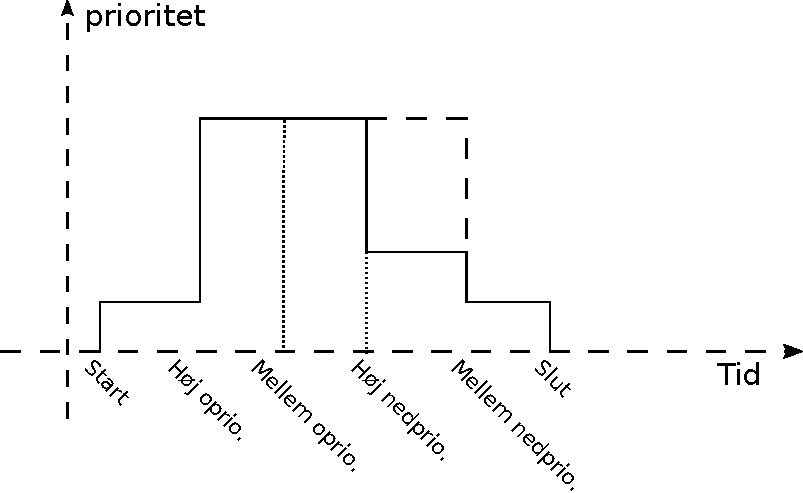
\includegraphics[scale=1]{images/priority-inheritance}
	\caption{Figuren viser hhv. forventet og faktisk prioritetsarvning. Der hvor den faktiske og forventede opførsel adskiller sig er forventet den fuldt optrukne streg, mens den stiplede streg er den faktiske opførsel.}
	\label{fig:priority-inheritance}
\end{center}
\end{figure}
  

\subsection{Slagterieksempel}

Først vil vi sammenligne de to udviklede versioner, for at se på deres fordele og ulemper, og til slut vi i dette afsnit sammenholde de to versioner, med et  eksempel der er implementeret i RTP-versionen.

Helt generelt opnår man når man ved brug af \pycsp et netværk, der nemt kan udvides hvis de fysiske rammer for slagteriet ændre sig. Viser det sig f.eks at kameraet holder den samlede produktivitet af netværket tilbage kan, slagteriet tilføjet endnu et kamera, og nemt udvide procesnetværket med endnu en kameraproces, som kan arbejde samtidigt med det første kamera. 

Forskellen i kode mellem \code{greenlets} og \code{proces}-versionen består af en linje, som indikerer hvilken version \pycsp skal bruge. En kørsel mellem de to versioner giver dog forskelligt resultat, som vist i \cref{tab:deadline-runs}. Dermed har valget af version betydning for både andelen af griseobjekter, der kan nå at blive bearbejdet, og hvor lang tid det tager i køre testen. Dette skyldes at testen køres på en multikerne CPU hvor \code{proces}-versionen dermed har mulighed for at køre parallelt. \code{Greenelts}-versionen derimod er begrænset til kørsel af en proces hvorfor der er flere grise der ikke når at blive bearbejdet inden for sin deadline.

\begin{table}[htbp]
	\centering
	\begin{tabular}{lrr}
       	\toprule
        \mc{Version} & \mc{Succesrate (\%)} & \mc{Tidsforbrug (s)} \\
        \midrule
        Greenlets & 42 & 16,5\\
        Processes & 71 & 10,3\\
        \bottomrule
    \end{tabular}
	\caption[]{Gennemførslen af simulation hvor 100 grise bliver sendt igennem procesnetværket. }\\
	\label{tab:deadline-runs}
\end{table}

Forskellen på kørselstiderne skyldes at detektoren venter på at aflevere griseobjektet til kameraet, og først når objektet er afleveret venter detektoren et normalfordelt tidsrum. Om dette er en urealistisk opførsel vil kræve mere domæneviden. Kan detektoren f.eks styre transportbåndet der fører grisene hen til detektoren er det en rimelig antagelse, mens det er urealistisk hvis båndet kører uafhængigt at detektoren.

I \code{procees}-versionen findes der fire processer og dermed kan der bearbejdes fire griseobjekter samtidigt. Dette sikre at det er de fire  griseobjekter nærmest robotten der arbejdes på, men samtidigt betyder det at man maksimalt kan arbejde på fire grise samtidigt. Ved at øge antallet af griseobjekter man kan arbejde på, vil man få mere tid per gris til at foretage de nødvendige beregninger. Man kan derfor vælge at tilføje flere konverterings og analyseprocesser, da disse ikke er bundet op på specialiseret hardware, og på den måde øge antallet af processer der kan arbejde samtidigt. Dette vil dog øge antallet af processer der må kæmper mod hinanden for CPU-tid, og griseobjekterne vil desuden skulle kæmpe mod hinanden for at komme igennem netværket uden hensyn til hvilken gris der er nærmest robotten. Man risikere dermed en starvation situation hvor griseobjekter svarende til  grise længere tilbage på transportbåndet overhaler griseobjekter længere fremme på transportbåndet.

\code{RTP}-udvidelsen bygger på \code{greenlets}-versionen, og vil derfor have de samme begrænsninger som denne, som diskuteret i implementeringen i afsnit \cref{sec:deadline-exampel-implementation}. Der er dog også en række fordele som vi vil komme ind på her.

Ved implementering af slagterieksemplet i \code{RTP}-versionen, slipper de enkelte processer for at holde styr på tiden, og vurdere om den enkelte gris deadline er overskredet. Når de modtager en gris sætter de deres egen deadline til grisens via funktionen \code{Set\_deadline}.  Hver proces skal i modsætningen til \code{greenlets}-versionen, kunne håndtere at modtage en \code{DeadlineException}, som de i dette eksempel blot kan håndteres ved at smide den nuværende griseobjekt væk. Det kan de gøre, da robotten på dette tidspunkt tager en beslutning uden specialviden om grisen, og griseobjektet er derfor ikke længere er relevant. I stedet kan processen  gå i gang med modtage et nyt griseobjekt.

I \code{greenlets}-versionen kom vi ind på at processerne frivilligt skal afgive kontrollen, før robotten kan foretage udskæringen, men at der ikke findes en metode til midlertidigt at afgive kontrollen. Med \code{RTP}-versionen og funktionen \code{Release} har alle processer mulighed for at afgive kontrollen så robotten rettidigt kan foretage selve udskæringen. Hermed skal vi ikke introducere en delt datastruktur.
  
selvom det var nødvendigt at basere RTP på  \code{greenlets}-versionen, medfører det at  kun en proces kan være aktiv på samme tid. Dermed kan vi kun udnytte en processor, som  passer dårligt sammen med denne applikation, som det ses af \cref{tab:deadline-runs}.  Vi kan dog til dels afhjælpe dette problem ved at udnytte at der i \code{greenlets}-versionen, findes en \code{IO}-dekorering. Denne dekorering placerer en funktion i en separat tråd, så flere funktioner kan køre samtidigt. Man skal her dog være opmærksom på at GIL'en stadig forhindre parallel udførsel. Eventuel parallel udførsel vil derfor kræve at koden i IO dekoreringen, kalder eksterne moduler som diskuteret i \cref{chap:csp}. Denne mulighed for parallel bearbejdning af flere processer vil dog  som i \code{processes}-versionen resultere i at processerne vil kæmpe mod hinanden om CPU-resurser. \code{RTP}-versionen har dog den store fordel at vi sikrer vi i modsætning til \code{proces}-versionen ikke risikere at griseobjekterne overhaler hinanden, men at netværket hele tiden har fokus på først at videresende griseobejektet nærmest robotten. \CRef{fig:pig-network3} viser hvordan netværket kan se ud med flere konverterings og analyse processer. 

\begin{figure}
 \begin{center}
  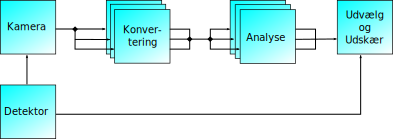
\includegraphics[scale=1]{images/pig-network3}
	\caption{Procesnetværk med flere konverteringsprocesser, og analyseprocesser}
	\label{fig:pig-network3}
\end{center}
\end{figure}

\section{Fremtidigt arbejde}
\section{Opsummering}
